\sys's design includes a novel task scheduler that uses efficient,
energy-aware task coalescing to amortize static task overheads, and uses a timer-based
task-splitting mechanism to avoid non-termination of tasks too long
for a device's energy buffer. 
% 
\subsection{Task Coalescing}
\label{sec:task_coalescing}
% 
When a device's buffered energy is sufficient to run multiple consecutive tasks
without a power failure, committing state after each task is an unnecessary
overhead. \sys eliminates this overhead by coalescing a sequence of tasks and deferring the commit
operations for all tasks to the end of the sequence. 
In general, committing involves moving state manipulated by a task
into its permanent location in non-volatile memory.  In particular, \sys's
commit procedure copies dirty pages of memory that a task updated between fast,
volatile working memory and slower, non-volatile main memory; we defer the
details of paging privatization and commit to Section~\ref{sec:memory_virtulaization}.

Coalescing tasks brings a double benefit. First, coalescing reduces the total number of relatively
high-latency, high-energy non-volatile memory accesses because tasks primarily
access variables in relatively low-latency, low-energy volatile memory.
Second, coalescing eliminates the unnecessary instructions that implement task
commit, which our measurements in Section~\ref{sec:evaluation} show constitute
a substantial run-time overhead.

An effective colescing strategy must be {\em aggressive} enough, attempting to coalesce a
large number of tasks to amortize a large amount of commit overhead. However, it must also be 
{\em conservative} enough, attempting to coalesce only as many tasks as will execute
to completion given a certain energy conditions, reducing the risk or long coalesced task re-execution penalty. 
%

\begin{algorithm}[t]
	\caption{Coalescing}
	\label{algo:genCoalescing}
	\scriptsize
	\begin{algorithmic}[1]
        \State $B \leftarrow $ \Call{$f_\text{reboot}$}{$z$}
        \State $H \gets 0$ 
        \While{$\texttt{true}$}       
	        \State $ i \gets 0$
	        %
	        \While{$ i <= B$}
		        \State \Call{execute\_task}{$T_\texttt{i}$}
		        \State $W \leftarrow $ \Call{$f_\text{weight}$}{$T_\text{i}$}
		        \State $i \gets i + W$
				\State $H \gets H + W$
	        \EndWhile
	        %
	        \State \Call{commit\_to\_fram}{\null}
	        \State $B \leftarrow $ \Call{$f_\text{commit}$}{$B$}
        \EndWhile
	\end{algorithmic}
\end{algorithm}
% 
\subsection{Task Coalescing Strategies} 
Algorithm~\ref{algo:genCoalescing} shows the general structure of a coalescing strategy. In the algorithm, $B$ (target budget) is total number of static tasks
that \sys will next attempt to coalesce. $T_\text{i}$ is the $i$th task
executed since the last power failure. $H$ (history) is the total number of
tasks between the last executed task and the power failure that preceding it.
$W_\text{i}$ is the {\em weight} of a task $T_\text{i}$.  A task's weight $W$ is an
arbitrary quantity associated with the task that represents its cost in time or
energy to execute; different coalescing strategies may apply different weights
to a task.  For example, a uniform weighting scheme sets the weight of each
task to one, making them all effectively equal in cost to the coalescing
algorithm.  A different policy might use a weighting scheme that sets a task's
weight equal to its run time relative to the task that executes for the
shortest duration, which has unity weight. 

Different coalescing strategies adhere mainly to the template in
Algorithm~\ref{algo:genCoalescing}, varying in only a few {\em characteristic
operations} that the algorithm leaves deliberately abstract.  A strategy's
reboot update function, $f_\text{reboot}$, updates $B$, the target budget,
after a reboot. A strategy's weight lookup function, $f_\text{weight}$, returns
the a task's weight.  A strategy's commit update function, $f_\text{commit}$,
updates $B$ after a successful commit. The following sections detail several
possible coalescing strategies that we developed for \sys, albeit not the only possible. In fact, our system allows developers to design their own strategy to implement and link to Coala’s task scheduler. 
% 
\subsubsection{Energy-Oblivious Coalescing (EO)}
\label{subsec:energyBlind}
% 
A very simple {\em energy-oblivious} coalescing strategy treats all tasks as
having unity weight and varies the size of a coalesced task linearly. In such a
scheme, the number of tasks to coalesce, $B$, increases by a constant $x$ when
a coalesced sequence of tasks commits, and decreases by the same constant $x$
when a coalesced sequence of tasks fails to complete, i.e., after a power
failure. The characteristic operations of the energy-oblivious strategy are: 
%
\begin{equation}
	\begin{split}
		f_\text{reboot}(B)  		&	 = B - x \\
		f_\text{weight}(T_\text{i}) & 	 =  1 \\
		f_\text{commit}(B) 			& 	 = B + x
	\end{split}
\end{equation}
%
The energy-oblivious strategy reacts slowly to the variation in the energy
required to execute different tasks and to the variation in the effective quantum of
energy available to the device. With the successful commit of each coalesced task sequence, the coalescing target increases.  Eventually, the target may be too high and a coalesced task
composed of only fewer tasks will commit without interruption by a power
failure.
%
The strategy then linearly decreases the coalescing target, eventually reaching a
coalescing target that allows completion.
%
A key limitation of this algorithm lies in the equality of the target decrease
in $f_\text{reboot}$ and the increase in $f_\text{commit}$.  Let us assume $x=1$. If, after $k$ successful commits the target must decrease to its original value $B-k$ due to an energy drop, this strategy requires $k$ successive power failures.
%
\subsubsection{Energy-Guided Coalescing (EG)}
\label{subsec:energyAware}
%
\begin{figure*}
    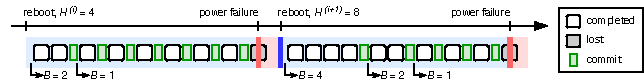
\includegraphics[width=\linewidth]{figures/hg-coal-horiz.pdf}
    \caption{HG coalescing sample execution across two power cycles. \textcolor{red}{explain the meaning of the letters and the logical connection between the left and the right (or cycle 1 and 2)}}
    \label{fig:hg-coal}
\end{figure*}
%
The \emph{Energy-Guided} (EG) coalescing strategy adapts its coalescing target more quickly, addressing a key limitation of the EO, to adhere to changes in energy conditions. It uses its recent execution history as 
mean to measure energy availability and alters its target accordingly.
By relying on the history of execution EG eliminates the problem of frequent power failures a single coalesced task. In fact EG can reduce its target to one from any coalesced target in at most two successive power failures. For instance, if the execution is interrupted after finishing a single task the history will be one ($H = 1$) and the target will be set to one also. 
While a history of $H$ suggests that there is sufficient energy to coalesce and
successfully commit $H$ tasks (i.e., to set $B = H$). EG conservatively sets $B$ equal to half of $H$ moderating the risk of a very long coalesced task. We experimented with a range of fraction values, settling on one half as the default for EG, because one half had the highest performance. The EG algorithm is characterized by the following functions: 
%
\begin{equation}
	\begin{split}
		 f_\text{reboot}(H) 			& = \lceil(H / 2)\rceil \\
		 f_\text{weight}(T_\text{i}) 	& =  1 \\
		 f_\text{commit}(B) 			& = \lceil(B / 2)\rceil
	\end{split}
\end{equation}
%
Fig.~\ref{fig:hg-coal} illustrates the operation of the EG.
The figure shows two power cycles following the $i$th, the latter having an
execution history $H^{(i)} = 4$.
Based on that, $B$ is initially set to two and then decreases to one. Once the
value of $B$ reaches one, EG is, in effect, expecting a power failure,
justifying the conservative approach. After the power failure, EG
uses the most recent history $H^{(i+1)} = 8$ to set $B = 4$
and continue execution.
%
\subsubsection{Weighted Energy-Guided Coalescing (WEG)}
\label{subsec:energyTaskAware}
%
The \emph{Weighted Energy-Guided} (WEG) coalescing strategy accounts for the
different energy and time cost of a program's tasks when setting the coalescing
target.
%
Each different task in the program consumes a different amount of energy to
execute to completion.  
%
The EO and EG coalescing strategies assume each task has uniform energy cost:
for these strategies, $B$ simply corresponds to a target {\em count} of tasks
coalesced, regardless of the individual cost of each task.
%
However, if one task executes for ten seconds and another executes for one
second, counting tasks misjudges the amount of {\em work} in the coalesced
tasks.

Instead, WEG associates a non-unity weight with each task in the program. 
%
WEG tracks the sum of the weights of tasks in a coalesced sequence of tasks.
%
When the sum of weights reaches $B$, the target, WEG commits the coalesced
task.
%
WEG differs from EO and HG by explicitly accounting for the variation in energy
cost of a program's tasks, eliminating the assumption that all tasks do the
same work, which is a key limitation.
%
WEG has the same characteristic operations as HG, except that
$f_\text{weight}(T_\text{i}) = W_\text{i}$.

The effectiveness of the WEG algorithm hinges on correctly identifying the
weight of each task, which WEG assumes is {\em statically} available.
%
Profiling the time and energy cost of tasks in a program is a difficult,
orthogonal problem~\cite{cleancut_2018,baghsorkhi_cgo_2018}.
%
WEG could use the result of an arbitrarily sophisticated profiling procedure.
%
To produce a concrete result in this paper, we give WEG access to a simple
profile of task run time collected offline using a single fixed input.
%
WEG stores the profile in a lookup table that maps a task's identifier to its
weight, making the information available to \sys's scheduler at run time.